\documentclass[10pt]{article}
\usepackage[a4paper,top=6mm,bottom=6mm,left=6mm,right=6mm,
            headheight=0pt,headsep=0pt,footskip=0pt]{geometry}
\usepackage[T1]{fontenc}
\usepackage{amsmath}
\usepackage{amssymb}
\usepackage{array}
\usepackage{xcolor}
\usepackage{tikz}
\usetikzlibrary{arrows.meta,decorations.pathreplacing}

% ================================================================
% Standard form flashcards.
%
% One card for each skill on the topic list, with a second card where
% a skill splits into different methods. Each card is written once,
% with \flashcard{<skill>}{<question>}{<answer>}, and \printflashcards
% lays them out twenty to a sheet, four across and five down: a page
% of questions followed by a page of answers.
%
% The answer page mirrors the columns, so that when the file is
% printed double-sided, flipping on the long edge, each answer lands
% on the back of its own question. The left and right margins are
% equal so that the cut lines meet on both sides of the paper. Both
% sides of a card carry its number, so a card can still be matched to
% its answer if the printer shifts the back by a millimetre or two.
%
% The answers use the wording of the Maths Revision topic list. A key
% fact from that sheet is set in bold with \key, and each card ends with
% the sheet's "Remember" line for its topic, set in bold purple with
% \remember to match the purple lines on the sheet.
%
% A card whose contents are too tall for it is drawn with a red frame
% and reported in the log as FLASHCARD OVERFLOW.
% ================================================================

\pagestyle{empty}
\setlength{\parindent}{0pt}
\setlength{\parskip}{0pt}
\setlength{\topskip}{0pt}

\newcommand{\fctopic}{Standard form}
\newcommand{\fccode}{SF}

% ----------------------------------------------------------------
% Card layout
% ----------------------------------------------------------------
\newlength{\fcw}\setlength{\fcw}{0.25\textwidth}
\newlength{\fch}\setlength{\fch}{56mm}
\newlength{\fcpad}\setlength{\fcpad}{2mm}
\newlength{\fciw}\setlength{\fciw}{\dimexpr\fcw-2\fcpad\relax}
\newlength{\fcgap}\setlength{\fcgap}{1.2mm}
\newlength{\fcspare}
\newlength{\fcbodytop}
\newsavebox{\fcheadbox}
\newsavebox{\fcbodybox}

% \flashcard{<skill>}{<question>}{<answer>} stores one card.
\newcounter{flashcard}
\newcommand{\flashcard}[3]{%
  \stepcounter{flashcard}%
  \expandafter\gdef\csname fcskill\arabic{flashcard}\endcsname{#1}%
  \expandafter\gdef\csname fcquestion\arabic{flashcard}\endcsname{#2}%
  \expandafter\gdef\csname fcanswer\arabic{flashcard}\endcsname{#3}}

% The idea a pupil must know to answer this type of question.
\newcommand{\key}[1]{{\bfseries\boldmath #1}}
% The quick way to remember the key step, worded as on the revision sheet.
\definecolor{remember}{RGB}{112,48,160}
\newcommand{\remember}[1]{{\color{remember}\bfseries\boldmath Remember: #1}}
% A line of working, centred and in display style. Used in place of \[ \],
% which leaves an empty line above it when it follows a paragraph break.
\newcommand{\working}[1]{\par{\centering$\displaystyle #1$\par}}

\newcommand{\fcquestionstyle}{\normalsize\raggedright\setlength{\parskip}{4pt}}
\newcommand{\fcanswerstyle}{\footnotesize\raggedright\setlength{\parskip}{2pt}}

% The strip across the top of a card: the skill on the front, and the
% card number on both sides.
\newcommand{\fcnumber}[1]{\makebox[10mm][r]{\color{black!55}\fccode\ #1}}
\newcommand{\fchead}[2]{%
  \begin{minipage}{\fciw}
    \scriptsize\color{blue!50!black}%
    \if#2Q\parbox[t]{\dimexpr\fciw-10mm\relax}{\raggedright\bfseries\csname fcskill#1\endcsname}%
    \else\textbf{Answer}\fi
    \hfill\fcnumber{#1}\par
    \vspace{0.6mm}%
    {\color{blue!30}\hrule height 0.4pt}%
  \end{minipage}}

% \fccard{<number>}{Q or A} draws one side of one card. Questions sit in
% the middle of the space under the strip; answers start at the top.
\newcommand{\fccard}[2]{%
  \sbox{\fcheadbox}{\fchead{#1}{#2}}%
  \sbox{\fcbodybox}{\begin{minipage}{\fciw}%
      \if#2Q\fcquestionstyle\csname fcquestion#1\endcsname
      \else\fcanswerstyle\csname fcanswer#1\endcsname\fi
    \end{minipage}}%
  \setlength{\fcbodytop}{\dimexpr\fcpad+\ht\fcheadbox+\dp\fcheadbox+\fcgap\relax}%
  \setlength{\fcspare}{\dimexpr\fch-\fcpad-\fcbodytop-\ht\fcbodybox-\dp\fcbodybox\relax}%
  \ifdim\fcspare<0pt
    \typeout{FLASHCARD OVERFLOW: \fccode\space #1 #2 by \the\dimexpr-\fcspare\relax}%
    \def\fccut{red}%
  \else
    \typeout{FLASHCARD SPACE: \fccode\space #1 #2 has \the\fcspare\space spare}%
    \def\fccut{black!35}%
    \if#2Q\addtolength{\fcbodytop}{0.5\fcspare}\fi
  \fi
  \begin{tikzpicture}
    \useasboundingbox (0,0) rectangle (\fcw,-\fch);
    \draw[line width=0.3pt,color=\fccut] (0,0) rectangle (\fcw,-\fch);
    \node[anchor=north west,inner sep=0pt] at (\fcpad,-\fcpad) {\usebox{\fcheadbox}};
    \node[anchor=north west,inner sep=0pt] at (\fcpad,-\fcbodytop) {\usebox{\fcbodybox}};
  \end{tikzpicture}}

\newcommand{\fctitle}[2]{%
  \hbox to \textwidth{\footnotesize\vrule width 0pt height 2.6mm depth 0.9mm
    {\color{blue!50!black}\bfseries\fctopic\ flashcards}\quad
    {\color{black!60}Sheet #1 of \fcsheets: \if#2Q questions\else answers\fi}\hfil
    {\color{black!60}Print double-sided, flipping on the long edge.}}%
  \vspace{1mm}}

% \fcpage{<sheet>}{Q or A}. On the answer page the columns run right to
% left, so that each answer is printed on the back of its question.
\newcommand{\fcpage}[2]{%
  \fctitle{#1}{#2}%
  \foreach \fcrow in {1,...,5}{%
    \nointerlineskip
    \hbox{\foreach \fccol in {1,...,4}{%
      \edef\fcn{\the\numexpr(#1-1)*20+(\fcrow-1)*4+\if#2Q\fccol\else(5-\fccol)\fi\relax}%
      \ifnum\fcn>\value{flashcard}%
        \hbox to \fcw{\vrule width 0pt height \fch\hfil}%
      \else
        \fccard{\fcn}{#2}%
      \fi}}}%
  \newpage}

\newcommand{\printflashcards}{%
  \pgfmathtruncatemacro{\fcsheets}{(\the\value{flashcard}+19)/20}%
  \foreach \fcsheet in {1,...,\fcsheets}{\fcpage{\fcsheet}{Q}\fcpage{\fcsheet}{A}}}

% ----------------------------------------------------------------
% Diagrams
% ----------------------------------------------------------------
% A calculator key, drawn as a small box.
\newcommand{\calckey}[1]{{\setlength{\fboxsep}{1pt}\fbox{\scriptsize #1}}}

\begin{document}

% ================================================================
% Writing numbers in standard form
% ================================================================
\flashcard{Writing large numbers in standard form}
{Write $4\,560\,000$ in standard form.}
{\key{Standard form $=$ (a number from 1 up to, but not including, 10) $\times\,10^{\text{power}}$}

One digit before the point: 4.56

{\centering
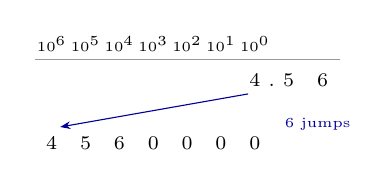
\begin{tikzpicture}[x=4.3mm,y=4mm,font=\scriptsize,every node/.style={anchor=base}]
  \foreach \p [count=\i from 0] in {6,5,4,3,2,1,0}{\node[font=\tiny] at (\i,1.1) {$10^{\p}$};}
  \draw[black!40] (-0.5,0.85) -- (8.5,0.85);
  \node at (6,0) {4}; \node at (6.5,0) {.}; \node at (7,0) {5}; \node at (8,0) {6};
  \foreach \d [count=\i from 0] in {4,5,6,0,0,0,0}{\node at (\i,-2) {\d};}
  \draw[-{Stealth[length=1.3mm]},blue!60!black] (5.8,-0.25) -- (0.25,-1.3);
  \node[font=\tiny,blue!60!black,anchor=west] at (6.6,-1.2) {6 jumps};
\end{tikzpicture}\par}

\working{4\,560\,000=4.56\times10^6}

\remember{One digit before the point, then count the jumps.}}

\flashcard{Writing small numbers in standard form}
{Write $0.000\,307$ in standard form.}
{\key{Small numbers (less than 1) have a negative power.}

One digit before the point: 3.07

{\centering
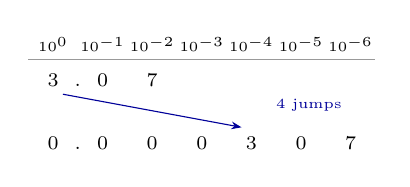
\begin{tikzpicture}[x=6.3mm,y=4mm,font=\scriptsize,every node/.style={anchor=base}]
  \node[font=\tiny] at (0,1.1) {$10^{0}$};
  \foreach \p in {1,...,6}{\node[font=\tiny] at (\p,1.1) {$10^{-\p}$};}
  \draw[black!40] (-0.5,0.85) -- (6.5,0.85);
  \node at (0,0) {3}; \node at (0.5,0) {.}; \node at (1,0) {0}; \node at (2,0) {7};
  \node at (0,-2) {0}; \node at (0.5,-2) {.};
  \foreach \d [count=\i from 1] in {0,0,0,3,0,7}{\node at (\i,-2) {\d};}
  \draw[-{Stealth[length=1.3mm]},blue!60!black] (0.2,-0.25) -- (3.8,-1.3);
  \node[font=\tiny,blue!60!black,anchor=west] at (4.3,-0.6) {4 jumps};
\end{tikzpicture}\par}

\working{0.000\,307=3.07\times10^{-4}}

\remember{One digit before the point, then count the jumps.}}

\flashcard{Standard form to ordinary numbers}
{Write $7.2\times10^5$ as an ordinary number.}
{\key{Big numbers have a positive power.}

$\times\,10^5$: the digits jump 5 places to the left. Fill the empty place values with zeros.
\working{\begin{aligned}
  7.2\times10^5&=7.2\times100\,000\\
               &=720\,000
\end{aligned}}

\remember{One digit before the point, then count the jumps.}}

\flashcard{Standard form to ordinary numbers}
{Write $5.9\times10^{-3}$ as an ordinary number.}
{\key{Small numbers (less than 1) have a negative power.}

$\times\,10^{-3}$ is $\div\,1000$: the digits jump 3 places to the right. Fill the empty place values with zeros.
\working{5.9\times10^{-3}=0.0059}

\remember{One digit before the point, then count the jumps.}}

% ================================================================
% Calculating in standard form
% ================================================================
\flashcard{Multiplying in standard form}
{Work out
\working{(3\times10^4)\times(6\times10^5)}
Give your answer in standard form.}
{\key{Multiplying: add the powers.}
\working{3\times6=18,\quad10^4\times10^5=10^9}
\working{(3\times10^4)(6\times10^5)=18\times10^9}
18 is not from 1 up to 10, so $18=1.8\times10^1$:
\working{18\times10^9=1.8\times10^{10}}

\remember{Numbers with numbers, powers with powers.}}

\flashcard{Dividing in standard form}
{Work out
\working{(2.4\times10^3)\div(6\times10^8)}
Give your answer in standard form.}
{\key{Dividing: subtract the powers.}
\working{2.4\div6=0.4,\quad10^3\div10^8=10^{-5}}
so the answer is $0.4\times10^{-5}$.

0.4 is less than 1, so $0.4=4\times10^{-1}$:
\working{0.4\times10^{-5}=4\times10^{-6}}

\remember{Numbers with numbers, powers with powers.}}

\flashcard{Adding and subtracting in standard form}
{Work out, giving your answers in standard form,

(a) $(4.2\times10^5)+(3.5\times10^4)$

(b) $(6\times10^{-3})-(4\times10^{-4})$}
{(a)
\working{\begin{aligned}
  420\,000+35\,000&=455\,000\\
                  &=4.55\times10^5
\end{aligned}}
(b)
\working{\begin{aligned}
  0.006-0.0004&=0.0056\\
              &=5.6\times10^{-3}
\end{aligned}}

\remember{Can't add powers: change to ordinary numbers first.}}

\flashcard{Standard form on a calculator}
{Use a calculator to work out
\working{\frac{4.68\times10^9}{7.2\times10^3}}
Give your answer in standard form.}
{4.68 \calckey{$\times10^x$} 9 \calckey{$\div$} 7.2 \calckey{$\times10^x$} 3 \calckey{$=$}

The display shows 650\,000:
\working{650\,000=6.5\times10^5}
Check: $4.68\div7.2=0.65$ and $10^9\div10^3=10^6$, so the answer is $0.65\times10^6=6.5\times10^5$.

\remember{Use the \calckey{$\times10^x$} key; it already includes the `$\times\,10$'.}}

% ================================================================
% Problems
% ================================================================
\flashcard{Speed, distance and time in standard form}
{Light travels at $3\times10^8$ metres per second. The Sun is $1.5\times10^{11}$ metres from the Earth.

How long does light from the Sun take to reach the Earth?}
{\key{Time $=\dfrac{\text{distance}}{\text{speed}}$}
\working{\frac{1.5\times10^{11}}{3\times10^8}=0.5\times10^3}
($1.5\div3=0.5$, $10^{11}\div10^8=10^3$)
\working{0.5\times10^3=5\times10^2\text{ s}}
That is 500 s, or 8 minutes 20 seconds (metres $\div$ metres per second gives seconds).

\remember{Right formula, numbers in, answer in standard form.}}

\flashcard{Population problems in standard form}
{The population of India is about $1.4\times10^9$. The population of Ireland is about $5\times10^6$.

How many times larger is the population of India?}
{How many times larger: divide the larger by the smaller.
\working{\frac{1.4\times10^9}{5\times10^6}=0.28\times10^3}
($1.4\div5=0.28$, $10^9\div10^6=10^3$)
\working{0.28\times10^3=2.8\times10^2}
India's population is about 280 times larger.

\remember{Right formula, numbers in, answer in standard form.}}

\printflashcards

\end{document}
